\section{\textbf{Ferramentas de desenvolvimento do projeto}}
\label{ferramentas-de-desenvolvimento-do-projeto}

Em relação as ferramentas de desenvolvimento, é notório que existe um trajeto amplo a ser percorrido pelos programadores. Isso ocorre porque existem várias linguagens de programação e \textit{frameworks} que auxiliam no desenvolvimento de sistemas. A escolha da melhor linguagem de programação e o melhor \textit{framework} para desenvolvimento depende muito do problema a ser resolvido e também das habilidades do programador. Há também um grande impasse na escolha da melhor linguagem e/ou do melhor \textit{framework}, que está relacionado a: interesses e aplicações comerciais; comunidade, para sanar possíveis duvidas e curva de aprendizado.

\subsection{{Linguagem de programação}}

Linguagem de programação são codificações escritas sequencialmente, seguindo uma estrutura assíncrona para a resolução de algum problema ou tarefa, que tem por finalidade ser compreendida por um computador. Essas codificações descrevem ao computador a sequência lógica de execução das funções e os comandos nos quais ele deve realizar para que a tarefa e/ou problema seja executado da melhor forma possível. Basicamente são divididas em linguagem de baixo nível e de alto nível, que significam, respectivamente, linguagens próximas ao entendimento de máquina ou \textit{hardware} (Binário ou hexadecimal) e linguagens próximas as linguagens naturais, ou seja, de fácil entendimento humano (\textit{While, if, write, read,} etc), nos quais são necessários compiladores para realizar a tradução, tornando possível a compreensão da máquina \cite{KELLEHER2005}.

Na busca por uma linguagem que poderia satisfazer e tornar possível a construção de uma solução para o impasse explícito no trabalho, fora identificado uma forte tendência na utilização do \textit{Python}.

\begin{comment}
De acordo com \citeonline{PILGRIM2009}, a projeção da linguagem enfatiza o trabalho do programador sobre o computacional, possibilitando assim a construção de bibliotecas e frameworks com uma facilidade acima do normal.

\textit{Python} foi criado por Guido van Rossum em 1991, com a ajuda de seus colegas Jack Jansen e Sjoerd Mullender. O objetivo deles era criar uma linguagem de fácil entendimento, orientada a objetos, menos complexa possível \cite{SONGINI2005}.

Segundo \citeonline{OLIVEIRA2007}, a linguagem sofreu vários ajustes no decorrer dos anos, tornando-se muito popular dentre os desenvolvedores e, consequentemente, dando início a inúmeras aplicações. Portanto, \textit{Python} é uma linguagem orientada a objetos, fortemente tipada, com propositos gerais de alto nível e de código aberto, objetivando uma construção ágil no desenvolvimento de aplicações. Sua sintaxe é bem simples e de fácil entendimento, reduzindo o custo de manutenção em \textit{softwares} criados a partir desta. Suas bibliotecas garantem ao programador um vasto acervo de funções que tem por finalidade facilitar o seu trabalho, reduzir tempo de codificação e evitar arquivos com extensas linhas de código. Devido à comunidade de código aberto, onde desenvolvedores tem acesso ao seu código fonte, a popularização da linguagem vem crescendo de forma significativa, visto que esta ainda não é muito conhecida \cite{SONGINI2005}.
\end{comment}

\subsubsection{\textit{Python}}

De acordo com \citeonline{PILGRIM2009}, a projeção da linguagem enfatiza o trabalho do programador sobre o computacional, possibilitando assim a construção de bibliotecas e frameworks com uma facilidade acima do normal.

\textit{Python} foi criado por Guido van Rossum em 1991, com a ajuda de seus colegas Jack Jansen e Sjoerd Mullender. O objetivo deles era criar uma linguagem de fácil entendimento, orientada a objetos, menos complexa possível \cite{SONGINI2005}.

Segundo \citeonline{OLIVEIRA2007}, a linguagem sofreu vários ajustes no decorrer dos anos, tornando-se muito popular dentre os desenvolvedores e, consequentemente, dando início a enumeras aplicações. Portanto, \textit{Python} é uma linguagem orientada a objetos, fortemente tipada, com propósitos gerais de alto nível e de código aberto, objetivando uma construção ágil no desenvolvimento de aplicações. Sua sintaxe é bem simples e de fácil entendimento, reduzindo o custo de manutenção em \textit{softwares} criados a partir desta. Suas bibliotecas garantem ao programador um vasto acervo de funções que tem por finalidade facilitar o seu trabalho, reduzir tempo de codificação e evitar arquivos com extensas linhas de código. Devido à comunidade de código aberto, onde desenvolvedores tem acesso ao seu código fonte, a popularização da linguagem vem crescendo de forma significativa, visto que esta ainda não é muito conhecida \cite{SONGINI2005}.

\subsubsection{{Biblioteca \textit{OpenCV}}}

Devido aos avanços em estudos científicos tecnológicos na área de visão computacional, o surgimento de bibliotecas que utilizam desta tecnologia evoluiu consideravelmente, proporcionando aos usuários maior versatilidade na escolha da melhor ferramenta para uma possível solução de seus problemas. Dentre as principais ferramentas que implementam algoritmos de visão computacional, pode-se citar as mais utilizadas: \textit{Matlab}, \textit{OpenCV} e \textit{scikit-image}. Este trabalho tem o objetivo de abordar apenas a biblioteca \textit{OpenCV}, no qual será utilizada para o desenvolvimento de uma possível resolução ao problema supracitado. A biblioteca \textit{Open Source} (Código aberto) está disponível no seu site oficial \citeonline{OpenCV}.

Desenvolvida pela Intel no ano 2000, escrita nativamente em C++, a biblioteca OpenCV permite a manipulação de dados de imagens, manipulações vetoriais, rotinas de álgebra linear, desenvolvimento de algoritmos de processamento de imagem, calibração de câmeras, dentre outros. Sua flexibilidade com várias linguagens de programação, como por exemplo o \textit{Python}, permite uma melhor integração com vários programas, evitando possíveis conflitos de incompatibilidade e proporcionando uma melhor flexibilidade no desenvolvimento de \textit{softwares} \cite{BARBOZA2009}.

A bilioteca possui certificação BSD - \textit{Berkeley Software Distribution}, representando que o software possui uma licença gratuita. A biblioteca contem mais de 2.500 algoritmos otimizados com diversas propriedades para resolverem problemas extensos. Há também vários setores de aplicação da biblioteca, visto que esta abrange diversas áreas como, por exemplo, reconhecimento de face e objetos, extração de modelos de objetos tridimensionais, união de imagens em uma única imagem, pesquisar por imagens semelhantes dentro de um banco de dados, acompanhar movimentos dos olhos, reconhecimento de cenários, dentre outros. No site oficial da ferramenta encontra-se dados nos quais informam que esta possui uma comunidade com mais de 47 mil usuários e um número estimado de download que ultrapassa a casa dos 18 milhões \cite{CUNHA2013}.

Segundo \citeonline{CUNHA2013}, um dos objetivos da biblioteca \textit{OpenCV} é fornecer uma infraestrutura robusta na área de visão computacional na qual seja de fácil manipulação, ajudando os desenvolvedores no processo de ampliação de aplicações sofisticadas de visão.

%\subsubsection{\textit{Framework}}

Atualmente, os projetos de desenvolvimento de \textit{software} aumentou consideravelmente. Devido a isso, programadores se deparam com um excesso de funções similares dentro dos vários projetos desenvolvidos no decorrer do tempo. Sendo assim, surgiu a necessidade de reutilizar códigos para poupar tempo. 

De acordo com \citeonline{JOHNSON97}, \textit{framework} são estruturas desenvolvidas com o objetivo de reutilizar tudo ou parte de um sistema representado por um conjunto de classes abstratas e concretas, ou seja,  uma estrutura parcialmente completa projetada para ser instanciada. Existe também \textit{frameworks}  que disponibilizam \textit{templates} como base para iniciar o desenvolvimento.

Os \textit{frameworks} disponibilizam para os desenvolvedores um vasto conjunto de bibliotecas, permitindo assim a realização de operações de grande porte. Sendo assim, os programadores focam mais em resolver problemas do que reescrever códigos, aumentando consideravelmente a produtividade da equipe. 

\subsection{{Ambientes virtuais}}

A virtualização vem sendo muito utilizada na área de desenvolvimento de \textit{software} devido à sua flexibilidade e fácil manipulação para realizar a criação de ambientes virtuais. Isso ocorre porque, com a virtualização, o usuário pode criar vários ambientes virtuais e, dentro deles, realizar a instalação das dependências necessárias para a execução do projeto. Portanto, o desenvolvedor pode ativar e desativar o ambiente virtual assim que necessário, sendo que as dependências do projeto estarão instaladas somente nesse ambiente, e não globalmente na máquina. Ou seja, as dependências do projeto serão desativadas assim que a virtualização for encerrada. A utilização de virtualização permite ainda que recursos computacionais possam ser alocados para múltiplas aplicações simultaneamente, sendo que cada uma dessas aplicações possui seu ambiente isolado das demais.

A situação citada acima é bastante válida se analisarmos o crescimento de ferramentas de programação disponíveis atualmente. Instalar vários \textit{frameworks}, pacotes de dependências de linguagens, bibliotecas e afins globalmente na máquina pode acarretar a lentidão, conflitos entre versões de linguagens de programação e \textit{frameworks} dos projetos, dentre outros. Quando isso acontece, por exemplo, em um projeto feito por uma equipe, a atualização de todas as dependências deve ser feita em todas as máquinas que estão envolvidas no projeto, para que a versão seja padrão em toda a equipe.

\subsection{{Sistema de controle de versões}}

Durante o processo de desenvolvimento de \textit{software}, a etapa de codificação gera várias linhas de códigos. Além disso, modificações e melhorias no \textit{software} ocorrem constantemente no decorrer do tempo, seja a pedido do usuário ou alguma possível atualização.  As equipes de desenvolvimento são compostas por vários tipos de desenvolvedores, cada um com sua personalidade e experiência. Sendo assim, os desenvolvimentos de \textit{softwares} são feitos por etapas, onde cada desenvolvedor é responsável por entregar o que foi designado a ele. 

Devido a isso, para organizar essas etapas de desenvolvimento, utiliza-se ferramentas que gerencia e controla diferentes versões de \textit{software}.  Segundo \citeonline{OReilly},  uma ferramenta que realiza o gerenciamento e o controle de versões de \textit{software} ou outro conteúdo “é referida genericamente como um VCS - \textit{Version Control System} (Sistema de controle de versão ), um SCM - \textit{Source Code Manager} (Gerenciador de código-fonte) ou um RCS - \textit{Revision Control System} (Sistema de controle de revisão)”. Essas ferramentas controlam quais linhas de códigos foram alteradas, qual contribuidor do projeto fez a alteração, o horário da alteração, dentre outros. Além do mais, essas ferramentas possibilitam aos desenvolvedores uma opção de voltar o código para versões anteriores, caso algum \textit{bug} (problema) na versão atual do sistema cause algum transtorno.

\citeonline{OReilly} enfatizam que nenhuma pessoa criativa e cautelosa inicia um projeto sem um método de \textit{backup}. Sendo assim, outra funcionalidade muito importante que as ferramentas de rastreamento e gerenciamento de código proporcionam para os desenvolvedores são os repositórios de \textit{backup}, que mantêm hospedado de forma segura todas os arquivos relacionados ao sistema desenvolvido.

\subsubsection{\textit{Git}}

Basicamente, o \textit{Git} é um sistema distribuído e de código aberto que controla versões de arquivos desenvolvidos, no qual possui diversos comandos que auxilia os desenvolvedores a realizar projetos de grade e pequeno porte com velocidade e eficiência.  Com esses comandos, o \textit{Git} disponibiliza um amplo conjunto de ferramentas para realizar a manipulação dos arquivos no seu repositório local ou \textit{Web}, garantindo a integridade dos dados \cite{GIT2010}.

A \autoref{fig_git} demostra um exemplo da utilização de comandos \textit{git} para controlar um repositório local ou \textit{web}.

\begin{figure}[h]
	\caption{\label{fig_git}Exemplo de comandos \textit{Git}.}
	\begin{center}
		\resizebox{1\linewidth}{!}{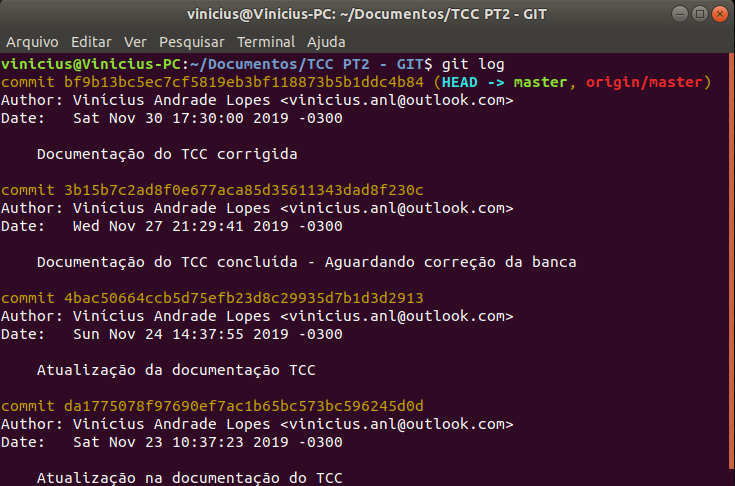
\includegraphics{4-Conteudo-Bibliografico/4-Ferramentas-de-Desenvolvimento-do-Projeto/git.png}}
	\end{center}
	\centering \legend{Fonte: Elaborada pelos autores.}
\end{figure}

Segundo \citeonline{CHACON2014}, o maior diferencial do sistema de controle de versões \textit{Git} é o seu modelo de ramificação (\textit{branch}), que possibilita ao usuário a criação de uma cópia do sistema principal. Com essa cópia, o desenvolvedor pode realizar implementações de melhorias/correções em trechos de códigos sem modificar a aplicação principal. Depois da implementação e dos testes, o desenvolvedor pode substituir a \textit{branch} principal (\textit{master}) pela \textit{branch} com implementações. Os únicos arquivos que serão substituídos serão os arquivos editados.

\subsubsection{\textit{GitHub}}


Já o \textit{GitHub} é uma plataforma de hospedagem de códigos que utiliza o \textit{Git} como controle de versão. O \textit{GitHub} possui uma grande interação com repositórios \textit{Git}, concentrando uma grande comunidade de desenvolvedores que colaboram para milhões de projetos \cite{CHACON2014}.

Ainda segundo \citeonline{CHACON2014}, o \textit{GitHub} hospeda a maior porcentagem de repositórios \textit{Git}. Isso ocorre porque a plataforma também disponibiliza recursos de gerenciamento de código, como por exemplo o rastreamento de problemas, revisão de código, edição \textit{online} do código, dentre outros.